\section{Алгоритм FP-Growth}
Алгоритм FP-Growth был опубликован в 2005 году Кристианом Боргельтом, и до сих пор является передовым в поиске ассоциативных правил. Алгоритм APriory, работает за $O(nl\cdot 2^k)$, где $n$ - это число признаков, $l$ - число записей в базе, а $k$ - максимальный размер ассоциативного правила. В то же время FP-Growth работает за $O(nl + f(k, n))$.

Идея этого алгоритма лежит в создании бора всех наборов $\varphi$, который будет хранить всю информацию о частотах встречаемости наборов, благодаря чему нам не придётся каждый раз пробегать всю базу с целью подсчёта $\nu(\varphi)$
\newline\newline
Алгоритм состоит из двух этапов:
\begin{enumerate}
    \item Построение FP-дерева
    \item Построение списка ассоциативных правил
\end{enumerate}

\subsection{Построение FP-дерева}

\begin{figure}[h]
    \centering
    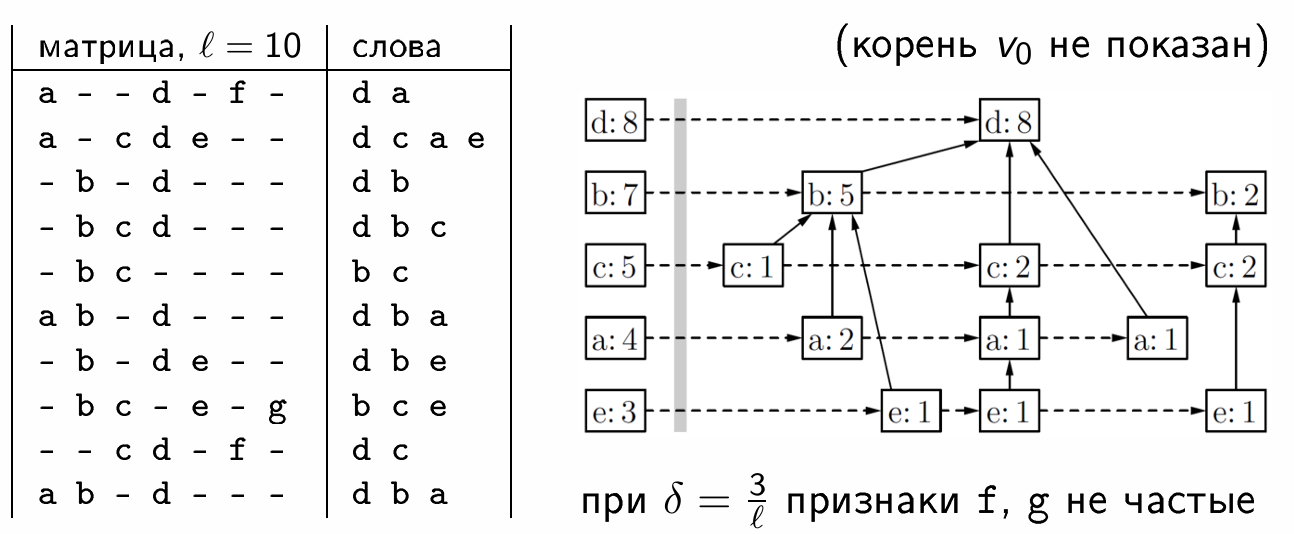
\includegraphics[width=0.8\linewidth]{chapters/metric/images/fp-tree-example.png}
    \caption{Пример FP-дерева}
\end{figure}

Первым делом упорядочим все признаки $f \in \mathcal{F}: \nu(f) \geq \delta$ по убыванию $\nu(f)$, их порядок будет соответствовать уровням вершин дерева (это не глубины!). Будем последовательно перебирать транзакции из базы. Будем хранить бор (FP-дерево), в каждой вершине $v$ которого будут храниться: 
\begin{enumerate}
    \item Признак $f_v \in \mathcal{F}$
    \item Множество дочерних вершин $S_v$
    \item Счетчик $c_v = \l\nu(\phi_v)$, где $\phi_v$ - набор состоящий из признаков соответствующих пути от корня до данной вершины. По сути этот счетчик равен количеству строк из базы, распознаваемых данной вершиной.
\end{enumerate}

Пусть для текущей транзакции $i$ положительны признаки из множества $F_i = \{f \in \mathcal{F}: f(x_i) = 1 \}$, упорядочим их по убыванию $\nu(f)$, получим строку $R_i$, начнем распознавать её бором. Если её нет в боре, создадим недостающие вершины, проинициализировав счетчики $c_{v_i} = 0$ в новых вершинах. Добавим 1 к счетчикам $c_v$ вершин, которые лежат на пути от корня, соответствующем $R_i$.

\begin{figure}[h]
    \centering
    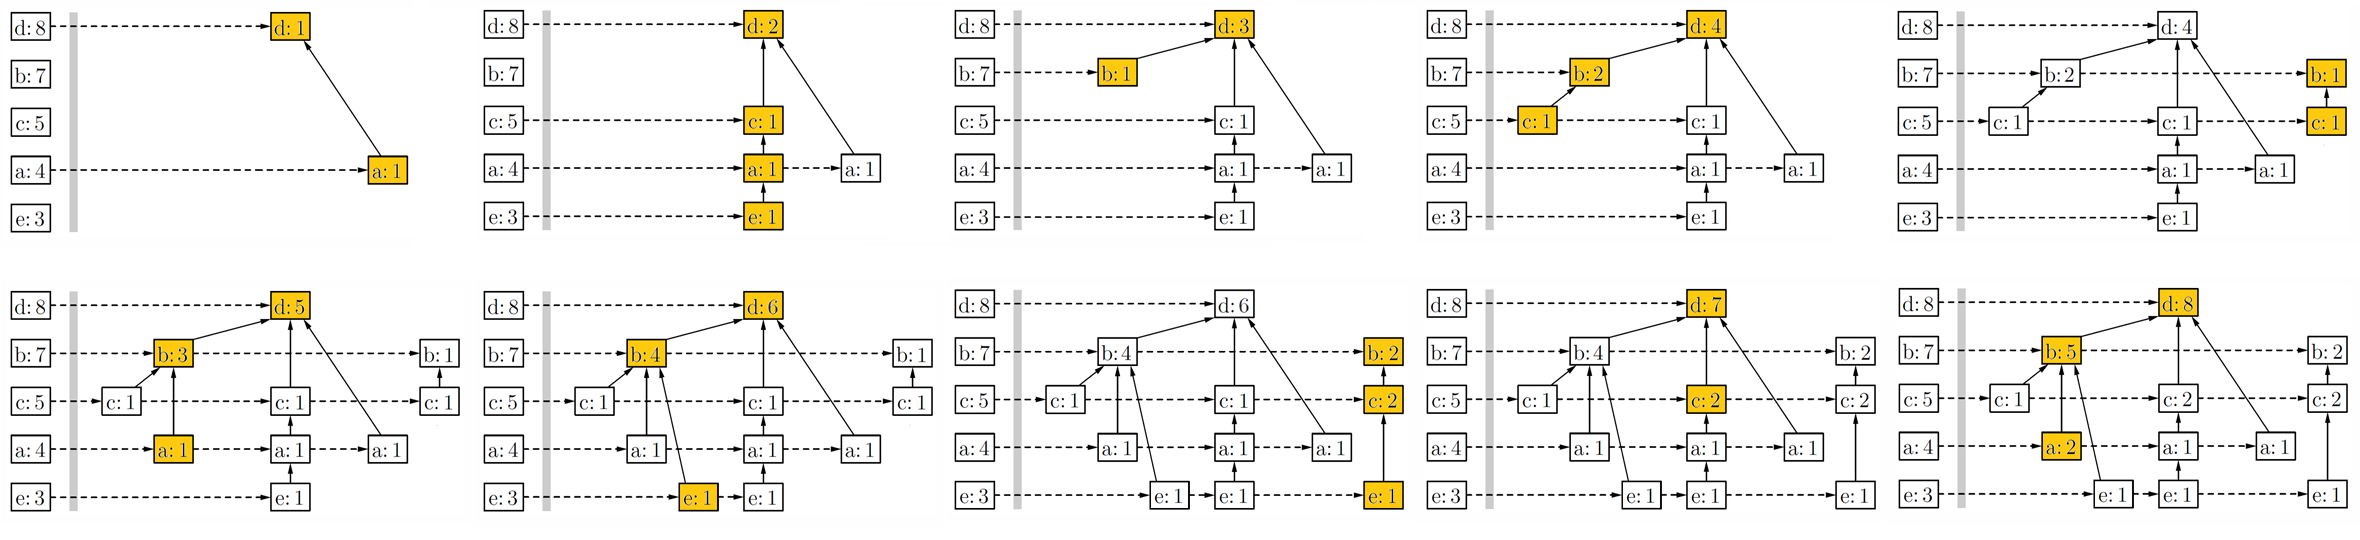
\includegraphics[width=1\linewidth]{chapters/metric/images/fp-tree-stages-example.png}
    \caption{Иллюстрация этапов построения FP-дерева}
    \label{fig:enter-label}
\end{figure}

\textbf{Введём обозначения:}

\begin{itemize}
    \item $V(T, f) = {v \in T: f_v = f}$ - все вершины, соответствующие признаку $f$. Соответственно, у них равные глубины.
    \item $C(T, f) = \displaystyle\sum_{v \in V(T, f)} c_v$ - Сумма счетчиков вершин, соответствующих признаку $f$. Несложно понять, что эта сумма равна числу объектов $x_i \in U$, для которых $f(x_i) = 1$. Другими словами $C(T, f) = l\nu(f)$
\end{itemize}


\subsection{Построение условного FP-дерева}

Прежде чем приступить к второму этапу алгоритма, разберёмся в одной важной для него процедуре. 
\newline\newline
\textbf{Определение.} Пусть FP-дерево $T$ построено по подвыборке $U$. Условное FP-дерево $T' = T|\varphi$ - это FP-дерево, порождаемое подвыборкой $\{x_i \in U| \varphi(x_i) = 1 \}$ из которого удалены все вершины признака $f$ и ниже.
\newline\newline
Рассмотрим алгоритм построения $T|f$ по $T$, где $f$ - признак из $\mathcal{F}$:
\begin{enumerate}
    \item Оставим в дереве только те вершины, которые принадлежат путям, идущим от вершин признака $f$ до корня. 
    \item Обновим счетчики $c_i$: для вершин признака $f$ ничего не меняем, а для остальных рекурсивно снизу вверх обновляем по формуле $c_u = \displaystyle\sum_{w \in S_u} c_w$
    \item Удаляем вершины признака $f$ из $T'$.
\end{enumerate}

Корректность следует из построения.

\subsection{Построение списка ассоциативных правил}

Для начала поймем, как эффективно находить $\nu(\varphi)$ используя FP-дерево. Для этого мы можем просто найти $f =argmin_{f \in \varphi} (\nu(f))$ и просуммировать $c_v$ для всех вершин $v$ признака $f$, таких что $\varphi \subset [f_{v_0}, f_{v}]$, где $[f_{v_0}, f_{v}]$ - набор признаков $f_{v_i}$ вершин из пути от корня до $v$.
\newline\newline
Рассмотрим функцию FP-find$(T,\varphi,R)$, которая находит по FP-дереву $T$, все частные наборы, содержащие только частный набор $\varphi$, и признаки, которые в FP-дереве стотят выше всех признаков из $\varphi$, и добавляет их в список $R$. Она играет ключевую роль в работе данного алгоритма. Вот как её можно реализовать:
\newline\newline
\textbf{Псевдокод:}

\noindent\hrulefill % Горизонтальная линия
\begin{enumerate}
    \item \textbf{ПРОЦЕДУРА} FP-find$(T,\varphi,R)$;
    \newline
    \quad \textit{Вход:} $T$ — FP-дерево, частный набор $\varphi$, список наборов $R$.
    \newline
    \quad \textit{Выход:} Добавить все частные наборы, содержащие $\varphi$ в $R$.
    \item \quad для всех $f \in \mathcal{F} : V(T,f) \neq \emptyset$ по уровням снизу вверх:
    \item \quad \quad если $C(T,f) \geq l\delta$ то:
    \item \quad \quad \quad набор $\varphi \cup \{f\}$ - частый, добавляем его в $R$;
    \item \quad \quad \quad $T':=T|f$ - условное FP-дерево;
    \item \quad \quad \quad FP-find$(T',\varphi \cup \{f\},R)$; - рекурсивно найти все частые наборы, содержащие $\varphi \cup \{f\}$
\end{enumerate}
\noindent\hrulefill % Горизонтальная линия
\newline\newline
Для получения списка всех частых наборов, мы можем просто запустить FP-find$(T,\emptyset,\emptyset)$. Алгоритм просмотрит все наборы в обратном лексикографическом порядке. Для выделения ассоциативных правил теперь можем запустить функцию AssocRules из алгоритма APriory.

\subsection{Задачи для практики}
\textbf{Задача 1.} Как используя FP-дерево, построенное по выборке $U$ найти а) самый частый набор, б) самый редкий набор?
\newline\newline
\textbf{Решение.} 
\newline
а) По свойству антимонотонности, один из наборов размера 1 будет самым часто встречаемым. Так как признаки в FP-дереве уже отсортированы по частоте, самым частым будет самый верхний. Сложность алгоритма получается равной $O(1)$.
\newline
б) Подмножество каждого пути из корня в FP-дереве соответствует какому-то набору. Также каждый набор, соответствующий строке в базе, соответствует какому-то пути в дереве. По свойству антимонотонности, одним из наборов, соответствующих путям из корня до листьев, должен быть самым редким. Количество упоминаний одного из таких наборов - это значение счетчика $c_v$ в соответствующем листе. То есть наша задача сводится к поиску листа с минимальным значением этого счетчика. Это можно сделать, пройдя обходом в глубину по всему дереву, за $O(2^n)$, где $n$ - глубина дерева в худшем случае.
\newline\newline
\textbf{Задача 2.} Как по уже построенному FP-дереву для выборки $U$ и фиксированных параметров поддержки $\delta$ и значимости $\chi$, найти все ассоциативные правила, удовлетворяющие $\delta, \chi$ вида $a \to b$, где $a,b \in \mathcal{F}$ за $O(n2^n)$ в худшем случае?
\newline\newline
\textbf{Решение.} 
\newline
Заметим, что всего таких правил порядка $n^2$, где $n$ - число признаков. То есть для того, чтобы дать ответ, нам достаточно найти $\nu(f), \nu(f \cup g)$ для всех признаков $f,g$ из дерева. Первые величины уже известны, так как были вычислены на первом этапе построения FP-дерева. Для нахождения всех $\nu(f \cup g)$, достаточно создать двумерный массив $C$, такой что $C_{fg}$ равно числу $x \in U: (f \wedge g)(x_i) = 1$. Для его заполнения мы можем пройти обходом в глубину по дереву, и находясь в вершине $v$, прибавлять $c_v$ к $C_{f_vf_u} = C_{f_uf_v}$ для всех $u \in [v_0, v]$, где $ [v_0, v]$ - путь от корня до $v$. Этот обход потребует порядка $O(n2^n)$ действий. То есть суммарно у нас уйдет $O(n2^n + n^2) = O(n2^n)$ действий.
\newline\newline
\textbf{Задача 3.}
Оцените время работы алгоритма FP-Growth для нахождения ассоциативных правил, удовлетворяющих поддержке $\delta$ и значимости $\chi$ в худшем случае.
\newline\newline
\textbf{Решение.} 
\newline
Если с временем построения FP-дерева все понятно - оно совпадает с временем построения бора по массиву строк и равно $O(nl)$. То асимптотика генерации всех частых наборов и выделение ассоциативных правил значительно труднее для вычисления. Построение условного FP-дерева $T|f$ по самому нижнему признаку $f$ выполняется одним обходом в глубину - асимптотически $O(2^n)$. Пусть FP-find$(T,\emptyset,\emptyset)$ выполняется за время $k(n)$, тогда $k(n) = O\left(\sum_{i = 0}^{n-1} (2^i + k(i))\right)$, где $2^i$ действий уходит на построение условного дерева по каждому из признаков. Сделаем замену $t(n):=2^n+k(n)$, тогда $t(n) - 2^n = O\left(\sum_{i = 0}^{n-1}t(i)\right)$, заметим, что для $t(n) = n2^n$ верно: $n2^n = O\left(\sum_{i = 0}^{n-1} i2^i\right) = O((n-2)2^n)$. Значит $k(n) = O(n2^n)$. Теперь найдем время выделения ассоциативных правил. Операция нахождения $\nu(\varphi)$ по данному $\varphi$ может быть оптимизирована с использованием дерева поиска для хранения множества $\varphi$, что даст суммарное время работы $O(nlogn + 2^d\cdot \log(n)) = O((2^d + n)\cdot \log(n))$, где $d$ - глубина самого нижнего признака из $\varphi$. Для выделение ассоциативных правил из набора $\varphi$ длинны $k$, время упирается в скорость вычисления $\nu(\varphi')$ для проверки $\nu(y' | \varphi') \geq \chi$, поэтому оно будет не хуже, чем $O(2^k \cdot (2^d + n)\cdot \log(n)))$, и не лучше $O(2^{k-1} \cdot (2^d + n)\cdot \log(n)))$ - так как есть $2^{k-1}$ набор содержащий признак глубины $d$, поддержку которого надо вычислить. Наконец выделение всех ассоциативных правил для всех частых наборов в худшем случае будет порядка 
$$O\left(\sum_{d = 1}^{n} \sum_{k = 1}^{n-d} \mathrm{C}_{n-d}^{k} \cdot 2^{k-d}\cdot \log(n) \right) =
O\left(\sum_{d = 1}^{n} \frac{3^{n-d}}{2^d} \cdot\log(n) \right) =O(3^n \log(n))  $$
Что и будет решающим слагаемым в асимптотике работы всего алгоритма.
